A análise de regressão é um conjunto de métodos estatísticos que buscam estimar a relação entre uma variável dependente $Y$ (também chamada variável resposta) condicionada a uma ou mais características explicativas $X$. O caso clássico dos métodos de regressão ajusta uma reta que minimiza o quadrado da diferença entre ela e os valores observados, em torno da qual se encontra uma distribuição de resíduos, conforme ilustrado na Figura \ref{fig:exemplo_regressao}.

\begin{figure}[H]
    \centering
    \caption{Dispersão de pontos com distribuições de $Y | X$}
    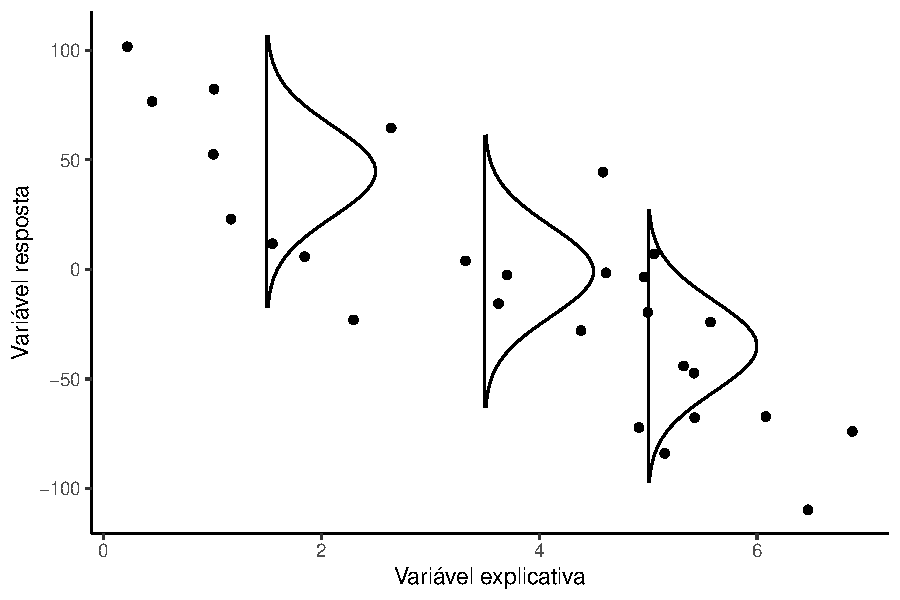
\includegraphics[scale=1.05]{imagens/scatter2.pdf}
    \label{fig:exemplo_regressao}
\end{figure}

 Os dois métodos que serão utilizados no estudo são a regressão gaussiana e a regressão quantílica, que estimam, respectivamente, a média condicional $E(Y|X)$ e os quantis condicionais $Q(Y|X)_\tau$.

\newpage
\subsection{Regressão Gaussiana}
A regressão gaussiana linear, regressão por mínimos quadrados ou simplesmente regressão linear, é um método que ajusta uma reta que para a esperança condicional $E(y_i|\mathbf{x}_i)$, minimizando a diferença quadrática entre ela e um conjunto de observações. Sejam $\varepsilon_i = y_i - E(y_i|\mathbf{x}_i)$ os resíduos do modelo, $\beta_0$ o coeficiente linear, $\beta_k$ os coeficientes angulares e $x_{ik}$ o valor da variável explicativa $k$ na observação $i$, para $k = 1, \dots, p$. Os pressupostos deste modelo são:

\begin{enumerate}
    \item $E(y_i|\mathbf{x}_i) = \beta_0 + \beta_1 x_{i1} + \dots + \beta_p x_{ip}$. A esperança $E(y_i|\mathbf{x}_i)$ pode ser descrita como uma combinação linear entre os parâmetros do modelo e as variáveis explicativas.
    \item $E(\varepsilon_i) = 0, \forall i$. Os erros têm média zero.
    \item $Var(\varepsilon_i) = \sigma^2, \forall i$. A variância dos erros é constante.
    \item $cov(\varepsilon_i, \varepsilon_j) = 0, \forall i \neq j$. Os erros são independentes entre eles.
    \item $\varepsilon_i \sim N(0, \sigma^2), \forall i$. Os erros têm distribuição normal.
\end{enumerate}

%Seja $\mathbf{x}$ um vetor de variáveis aleatórias independentes e $\varepsilon$ um vetor de erros aleatórios, onde $\varepsilon_i$ satisfaz a propriedade de ser normalmente distribuído, com média $\mu = 0$ e variância $\sigma_i ^ 2$ constante para cada $\varepsilon_i$, qualquer que seja o valor de $x_i$ ($i \in \{1, \dots, n\}$).

% Seja $Y$ uma variável resposta. A regressão gaussiana ajusta um vetor de coeficientes $\beta$ de uma equação
%\begin{equation}
%Y = \mathbf{\beta ^ {T} x + \varepsilon}.
%\end{equation}

Dada uma matriz $\mathbf{X}$  de valores observados ordenados das variáveis explicativas e $\mathbf{y}$ um vetor de valores observados da variável resposta, é possível demonstrar que, satisfeitos os pressupostos do modelo, o vetor de coeficientes $\hat{\beta}$ na forma

\begin{equation}
\hat{\beta} = (\mathbf{X}^{T}\mathbf{X})^{-1} \mathbf{X}^{T} \mathbf{y},
\end{equation}

\noindent constitui um estimador consistente e não-viesado de variância mínima do vetor de parâmetros $\beta$ \cite{kutner}.

Para verificar se os parâmetros são significativos, é possível construir as hipóteses

$$H_0: \beta_1 = \beta_2 = \dots = \beta_n = 0,$$
$$H_1: \text{Pelo menos um } \beta_i \neq 0, i = {1, \dots, p},$$

\noindent cuja estatística de teste

\begin{equation}
\frac{\frac{1}{p-1} \sum(\hat{y}_i - \bar{y})^2}{\frac{1}{n-p}\displaystyle \sum_{i=1}^n \varepsilon_i^2} = \frac{MS_R}{MS_E}
\end{equation}

\noindent tem distribuição $F(p-1, n-p)$ sob $H_0$, onde $p$ é o número de parâmetros estimados do modelo e $n$ e o número de observações dos dados.

\subsection{Regressão Quantílica}
Diferente do modelo de regressão gaussiana, que traça a reta para a média de uma variável resposta dependente de variáveis explicativas, a regressão quantílica traça a reta para qualquer quantil condicionado a $\mathbf{X}$, tornando-a mais robusta que o modelo de mínimos quadrados no que se refere à influência de outliers.

A regressão quantílica depende de menos pressupostos que o modelo por mínimos quadrados, pois não assume normalidade e variância constante dos erros. A regressão quantílica assume que os erros são não-correlacionados entre eles e $Q_\tau(\varepsilon_\tau | \mathbf{X}) = 0$. Embora modelos quantílicos não-lineares também sejam possíveis, este trabalho assumirá que as relações entre as variáveis são lineares.

O $\tau$-ésimo quantil de uma distribuição de probabilidades é qualquer ponto $y$ da variável aleatória tal que a probabilidade de um valor ser menor ou igual a $y$ é igual a $\tau$. Considerando $F(y)$ a função de distribuição acumulada da variável aleatória $y$, temos que

\begin{equation}
\tau = P(Y \leq y) = F(y).
\end{equation}

No caso empírico, convenciona-se o uso do valor mínimo do intervalo, de modo que a definição para o quantil assume a forma
\begin{equation}
F^{-1}(\tau) = \text{inf}\{y: F(y) \geq \tau\}.
\label{empirical_quantile}
\end{equation}

A distribuição empírica permite reduzir a estimativa para o quantil segundo métodos de otimização da função de perda \textit{pinball}, ou perda quantílica, expressa em

\begin{equation}
\rho_\tau(u) = u(\tau - I(u < 0)), \tau \in (0, 1),
\label{pinbal_loss}
\end{equation}

\noindent onde $I(u < 0)$ é uma função indicadora que assume valor 1 se a condição for satisfeita ($u < 0$) e valor 0, caso contrário. Segue que

\begin{equation}
    E\rho(X - \hat{x}) = (\tau - 1) \displaystyle \int_{-\infty}^{\infty} (x - \hat{x}) dF(x) + \tau \displaystyle \int_{\hat{x}}^{\hat{x}} (x-\hat{x}) dF(x).
\end{equation}

Calculando a derivada em relação a $\hat{x}$, e igualando a zero, teremos

\begin{equation}
    0 = \frac{d}{d\hat{x}} E\rho(X - \hat{x}) = (1 - \tau) \displaystyle\int_{-\infty}^{\hat{x}} dF(x) -\tau\displaystyle\int_{\hat{x}}^{\infty} dF(x) = F(\hat{x}) - \tau,
\end{equation}

\noindent de modo que a expressão \ref{pinbal_loss} encontra seu ponto de mínimo em qualquer elemento de ${x: F(x) = \tau}$, ou $\hat{x} = F^{-1}(\tau)$. Em caso de uma solução não-única, ou seja, de haver um intervalo de valores que satisfazem a condição, convenciona-se, como já mencionado em \ref{empirical_quantile}, que deve ser selecionado o menor dos valores deste intervalo.

Os métodos de otimização podem ser implementados computacionalmente através de algoritmos de otimização. Assim, encontra-se o $\hat{x}$ que minimiza

\begin{equation}
\displaystyle \min_{\xi \in \mathbb{R}} \displaystyle \sum_{i=1}^{n} \rho_\tau(y_i - \xi).
\label{problema_1}
\end{equation}

Analogamente, podemos reduzir o problema da regressão quantílica a um problema de otimização. Segue que o resultado deve resolver

\begin{equation}
\displaystyle \min_{\beta \in \mathbb{R}^{p}} \displaystyle \sum_{i=1}^{n} \rho_\tau(y_i - x_i^{\text{T}}\beta).
\label{problema_2}
\end{equation}

Segundo \citeonline{koenker2005}, é possível solucionar \ref{problema_1} através de uma expressão de programação linear, adicionando $2n$ variáveis artificiais $\{u_i, v_i: 1, \dots, n\}$, onde
\begin{equation}
    u_i = (y_i - \hat{y}_i) I(y_i - \hat{y}_i > 0)
\end{equation}
\begin{equation}
    v_i = (y_i - \hat{y}_i) I(y_i - \hat{y}_i < 0),
\end{equation}

\noindent que representam, respectivamente, as partes positivas e negativas do vetor de resíduos, com $I$ sendo uma função indicadora que assume valor 1 se a condição for satisfeita e 0, caso contrário. Note que $u_i$ e $v_i$ não podem ser simultaneamente diferentes de zero. Assim, a solução para \ref{problema_1} pode ser dada através de

\begin{equation}
    \displaystyle \min_{(\xi, u, v) \in \mathbb{R} \times \mathbb{R}_+ ^ {2n}} \{\tau \mathbf{ 1 _n ^ T u} + (1 - \tau) \mathbf{ 1_n ^ T v} | \mathbf{1_n}\xi + \mathbf{u - v = y}\},
\end{equation}

\noindent onde o elemento $\tau \mathbf{ 1 _n ^ T u} + (1 - \tau) \mathbf{1_n ^ T v}$ pode ser enunciado como o somatório dos erros ponderados pelo quantil (a função objetivo a ser minimizada) e $\mathbf{1_n}\xi + \mathbf{u - v = y}$ é a restrição. Analogamente, \ref{problema_2} pode ser resolvido com o programa linear

\begin{equation}
    \displaystyle \min_{(\beta, u, v) \in \mathbb{R} ^ p \times \mathbb{R}_+ ^ {2n}} \{\tau \mathbf{ 1 _n ^ T u} + (1 - \tau) \mathbf{ 1_n ^ T v} | \mathbf{X}\hat{\beta} + \mathbf{u - v = y}\},
\end{equation}

\noindent onde $\mathbf{X_{n\times p}}$ é a matriz de design e $\hat{\beta}$ é o vetor de coeficientes de regressão condicionado a $\tau$. Uma vez resolvido o problema de programação linear, a função quantil condicional $Q_\tau(\mathbf{y | X})$ pode ser expressa na forma

\begin{equation}
Q_\tau(\mathbf{y | X}) = \hat{\beta}_0(\tau) + x_1 \hat{\beta}_1(\tau) + \dots + x_p \hat{\beta}_p(\tau)  = \hat{\beta} (\tau) \mathbf{x}
\end{equation}

\noindent onde cada $x_{i}$, com $i \in \{1, ..., p\}$, é uma variável explicativa, e $Q_\tau(\mathbf{y | X})$ é o quantil condicional $\tau$ de $\mathbf{y}$ dado $\mathbf{X}$  \cite{koenker2005}. 

Para casos homoscedásticos, uma abordagem com a regressão gaussiana também seria capaz de traçar retas quantílicas através da função de distribuição dos resíduos, o que a tornaria preferível, uma vez que é mais eficiente computacionalmente, possui formas fechadas para os estimadores dos coeficientes de regressão e não dependeria de uma estimativa para cada quantil. Todavia, se a variação do $\beta(\tau)$ for grande em função de $\tau$, significa que os erros não são identicamente distribuídos, tornando a abordagem de regressão quantílica preferível, uma vez que não depende da suposição de homoscedasticidade que não foi satisfeita para o modelo de regressão gaussiana.

\subsubsection{Inferência para os coeficientes do modelo de regressão quantílica}
A inferência sobre os coeficientes de regressão quantílica pode ser feita de muitas maneiras. \citeonline{koenker2005} apresenta três métodos, sendo um baseado em resultados assintóticos (que será o foco neste trabalho), outro em bootstrap e, por fim, um teste baseado em escores ordinais. \citeonline{bassettkoenker} demonstraram o resultado que permite a inferência pela distribuição assintótica dos estimadores, como exposto no Teorema \ref{teo:distribuicao_assintotica_betas}.


\begin{teo}
\label{teo:distribuicao_assintotica_betas}

Seja $\{\hat{\beta_1}(\tau_1), \dots, \hat{\beta_M}(\tau_M)\}$, onde $0 < \tau_1 < \dots < \tau_M < 1$, uma sequência de vetores estimados para os coeficientes de regressão quantílica. Seja $\mathbb{\xi}(\tau) = F^{-1}(\tau)$ o quantil de nível \tau. Assuma que:

\begin{enumerate}
    \item $F$ é contínua e tem densidade contínua positiva $f$ em $\xi(\tau_i)$;
    \item Uma das colunas da matriz $\mathbf{X}$ é uma coluna de números 1;
    \item $\displaystyle \lim_{n\to\infty} \frac{1}{n}\mathbf{X^TX = Q}$, uma matriz positiva definida.

\end{enumerate}


Então,
$$\sqrt{n} [\hat{\beta}(\tau_1) - \beta(\tau_1), \dots, \hat{\beta_m}(\tau_M) - \beta_m(\tau_M)] \xrightarrow{D} N_M p(\mathbf{0}, \Omega(\tau_1, \dots, \tau_m; F) \otimes \mathbf{Q^{-1}}),$$

\noindent onde $\Omega$ é a matriz de covariância dos $M$ quantis amostrais das amostras aleatórias da distribuição F.

\end{teo}


Dessa forma, $\hat{\beta}(\tau)$ é um estimador não-viesado de $\beta(\tau)$. Seja $F = diag(f_1(0), \dots, f_n(0))$. Segundo \citeonline{kocherginsky2005}, caso os erros $e_i$ sejam independentes, sem necessariamente serem identicamente distribuídos, o estimador  

\begin{equation}
V(\tau) = \tau (1 - \tau )\mathbf{(X ^ T F X) ^{-1} (X ^ T X)(X ^ T F X) ^ {-1}}
\label{equation:asympt_var_beta}
\end{equation}

\noindent tende assintoticamente à matriz assintótica de covariâncias de $\hat{\beta}(\tau)$. Segundo \citeonline{brunoramodossantos}, é possível estimar $f_i(0)$ pela expressão

\begin{equation}
\frac{2h_n}{
    \mathbf{x}_i ^ \mathbf{T} \hat{\beta}_{\tau+h_{n}}-\mathbf{x} ^ \mathbf{T}_i\hat{\beta}}_{\tau-h_{n}}   
\label{f0_estimate}
\end{equation}

\noindent onde $\lim_{n\to\infty}h_n = 0$. Métodos para o cálculo de $h_n$ foram apresentados por \citeonline{hall_and_sheather_1988} citado em \citeonline{brunoramodossantos} e discutidos por \citeonline{koenker2005}. A opção de cálculo dos erros padrão \texttt{se="nid"}, do método \texttt{summary.rq} da biblioteca \texttt{quantreg} (em R) implementa a estimação através das expressões (\ref{equation:asympt_var_beta}) e (\ref{f0_estimate}).

Esses resultados assintóticos permitem a construção de intervalos de confiança e testes de hipóteses para os valores de $\beta(\tau)$. É possível aplicar um teste  para a hipótese linear geral aos modelos de regressão quantílica, através do qual se pode verificar

$$H_0: \beta_1(\tau) = \beta_2(\tau) = \dots = \beta_n(\tau) = 0,$$
$$H_1: \text{Pelo menos um } \beta_i(\tau) \neq 0, i \in {1, \dots, n},$$
\noindent cuja estatística do teste é
\begin{equation}
    T_n = n\displaystyle \sum_{i=2}^p \frac{\hat{\beta}_i^2(\tau)}{Var(\hat{\beta}_i(\tau))},
\end{equation}

\noindent que possui distribuição $\chi^2_{p-1}$ \cite{brunoramodossantos}.

\subsection{Seleção de variáveis}
Ao trabalhar com volumes grandes de dados, métodos para selecionar modelos se tornam relevantes, de forma que evitem tanto a simplificação excessiva quanto o sobreajuste. Para isso, existem métricas que verificam a qualidade do ajuste, tais como o Critério de Informação de Akaike (AIC), e o Critério de Informação Bayesiano (BIC).

\begin{equation}
AIC_p = 2p - 2 \log \hat{L} 
\end{equation}
\begin{equation}
    BIC_p = (\log n)p - \log \hat{L}
\end{equation}

Em ambas as métricas, quanto menor o valor resultante, maior é a qualidade do ajuste, com uma penalização baseada no número $p$ de variáveis incluídas no modelo. Para $n \geq 8$, temos $\log n \geq 2$, de forma que o BIC, para esses casos, tem uma penalização maior para o número de variáveis que o AIC, favorecendo modelos mais parcimoniosos \cite{kutner}.

Para a regressão gaussiana, $\hat{L}$ pode ser calculado através do $MSE_p$ \cite{montgomerylra}. Para a regressão quantílica, essa verossimilhança é calculada na forma $\frac{1}{n}\displaystyle\sum_{i = 1} ^ {n} \rho_{1/2}(y_i - x_i^{T}\hat{\beta_n}(1/2))$ \cite{koenker2005}. As métricas não têm uma interpretação direta, e pelo fato de os modelos possuírem funções de verossimilhança diferentes, elas não podem ser utilizadas para comparar modelos de diferentes tipos. Assim sendo, não é possível comparar o modelo quantílico com o modelo gaussiano utilizando AIC ou BIC, por exemplo.

\subsubsection{Regressão por \textit{stepwise}}
Uma comparação completa testaria todos os modelos possíveis e escolheria, dentre eles, o que otimiza a critério de seleção. Porém, conforme o número de variáveis aumenta, essa comparação se torna computacionalmente inviável, e se faz necessário o uso de algum procedimento de seleção automática. Os principais métodos são:

\begin{itemize}
    \item \textbf{Seleção \textit{forward}}: O modelo inicia sem variáveis preditivas, adicionando uma a cada passo através do critério inicialmente estabelecido, omitindo e removendo casos onde a variável adicionada não foi significativa.
    \item \textbf{Eliminação \textit{backward}}: O modelo inicia com todas as potenciais variáveis preditoras, e a cada passo, remove a variável menos relevante segundo o critério estabelecido.
\end{itemize}

Dessa forma, nem todos os modelos possíveis são testados, mas o modelo resultante do procedimento é um modelo que satisfaz os critérios \cite{kutner}. Os dois procedimentos podem ser combinados, resultando no \textit{stepwise} bidirecional, onde, a cada passo, é possível adicionar e remover variáveis. No software \texttt{R}, a biblioteca \texttt{MASS} disponibiliza as três opções de seleção através do método \texttt{stepAIC}, bastando definir o argumento \texttt{direction} como \texttt{"forward"}, \texttt{"backward"} ou \texttt{"both"}.
